% Status deck: précis + autocatpath — grounded, untiring research collaboration
% Build: tectonic slides.tex   (or pdflatex, twice)
% UL palette (dark mode): UL Green #00B140 (fills/dots), bright green #2BD877
% for headings/accents, on near-black #0E1412 with #D5DBD7 body text — swap freely.
% Maturity dots: \sdone = deployed & running · \srough = built, rough · \sidea = concept
% Per-frame citation footer: \citefield{...} inside the frame ('' to clear).
\documentclass[aspectratio=169,10pt]{beamer}
\usepackage[utf8]{inputenc}
\usepackage[T1]{fontenc}
\usepackage{tikz}
\usetikzlibrary{positioning,arrows.meta}
\usepackage{booktabs}

% beamer preloads hyperref — just style it; \doi{} makes clickable DOI links
\hypersetup{colorlinks=true,urlcolor=ULGreenBright,linkcolor=LightText}
\newcommand{\doi}[1]{\href{https://doi.org/#1}{\texttt{doi:#1}}}

% ---------- UL palette (dark mode) ----------
\definecolor{ULGreen}{HTML}{00B140}
\definecolor{ULGreenBright}{HTML}{2BD877}
\definecolor{DarkBG}{HTML}{0E1412}
\definecolor{LightText}{HTML}{D5DBD7}
\definecolor{MutedGray}{HTML}{93A09A}

\usetheme{default}
\setbeamercolor{background canvas}{bg=DarkBG}
\setbeamercolor{normal text}{fg=LightText,bg=DarkBG}
\setbeamercolor{frametitle}{fg=ULGreenBright}
\setbeamercolor{title}{fg=ULGreenBright}
\setbeamercolor{structure}{fg=ULGreenBright}
\setbeamercolor{author}{fg=LightText}
\setbeamercolor{institute}{fg=LightText}
\setbeamercolor{date}{fg=LightText}
\setbeamerfont{frametitle}{series=\bfseries,size=\large}
\setbeamertemplate{navigation symbols}{}
\setbeamertemplate{itemize items}{\textcolor{ULGreen}{\rule[0.4ex]{0.8ex}{0.8ex}}}

% ---------- maturity dots ----------
\newcommand{\sdone}{\tikz[baseline=-0.55ex]\fill[ULGreen] (0,0) circle (3.0pt);}
\newcommand{\srough}{\tikz[baseline=-0.55ex]{\fill[ULGreen!35!DarkBG] (0,0) circle (3.0pt);\draw[ULGreen,line width=0.8pt] (0,0) circle (3.0pt);}}
\newcommand{\sidea}{\tikz[baseline=-0.55ex]\draw[MutedGray,line width=0.8pt] (0,0) circle (3.0pt);}

% ---------- citation field + footline ----------
\gdef\SlideCite{}
\newcommand{\citefield}[1]{\gdef\SlideCite{#1}}
\setbeamertemplate{footline}{%
  \leavevmode%
  \hbox{%
    \begin{beamercolorbox}[wd=0.34\paperwidth,ht=2.4ex,dp=1.2ex,leftskip=1.5ex]{normal text}%
      \tiny \sdone~running\quad \srough~built, rough\quad \sidea~concept%
    \end{beamercolorbox}%
    \begin{beamercolorbox}[wd=0.44\paperwidth,ht=2.4ex,dp=1.2ex,center]{normal text}%
      \tiny \textcolor{MutedGray}{\SlideCite}%
    \end{beamercolorbox}%
    \begin{beamercolorbox}[wd=0.22\paperwidth,ht=2.4ex,dp=1.2ex,rightskip=1.5ex plus1fil]{normal text}%
      \hfill\tiny
      \IfFileExists{logos/ul-macatamo.png}%
        {\raisebox{-0.6ex}{\includegraphics[height=2.8ex]{logos/ul-macatamo.png}}}%
        {\textcolor{ULGreenBright}{\textbf{UL\,\textperiodcentered\,MACATAMO}}}%
      ~~\textcolor{MutedGray}{\insertframenumber}%
    \end{beamercolorbox}}%
}

\title{\texorpdfstring{\textbf{Précis + autocatpath}}{Precis + autocatpath}}
\subtitle{Grounded, untiring research collaboration --- status}
\author{Reto Stamm}
\institute{University of Limerick}
\date{August 2026}

\begin{document}

% ---------- 1 · title ----------
\begin{frame}
  \citefield{}
  \titlepage
  \begin{center}
    \small\textcolor{ULGreenBright}{``Grounded claims, not fluent guesses ---
    every assertion traced\\
    to a paragraph, a calculation, or a measurement,\\
    and an untiring machine to keep checking.''}
  \end{center}
\end{frame}

% ---------- 2 · hallucinations: origins ----------
\begin{frame}{Hallucinations: where they come from}
  \citefield{\href{https://doi.org/10.1038/s41586-024-07421-0}{Farquhar et al., Nature 630, 625--630 (2024)}}
  \begin{itemize}
    \item LLMs answer from the training distribution, not from evidence ---
          fluent guesswork whenever the evidence is thin
    \item Confabulation is measurable: semantic entropy separates
          ``knows'' from ``making it up''
    \item Retrieval alone does not fix it --- retrieved $\neq$ verified support
          for the claim actually made
  \end{itemize}
\end{frame}

% ---------- 3 · model collapse ----------
\begin{frame}{How fast it degrades: the model eats its own output}
  \citefield{\href{https://doi.org/10.1038/s41586-024-07566-y}{Shumailov et al., Nature 631, 755--759 (2024)} \(\cdot\) \href{https://arxiv.org/abs/2404.01413}{Gerstgrasser et al.\ (2024)}}
  \begin{itemize}
    \item Models fed their own generations degrade within a few
          generations --- rare knowledge (the tails) vanishes first
    \item Collapse is progressive and self-reinforcing without fresh,
          grounded data
    \item The antidote is small: keep \emph{accumulating} real data
          alongside the synthetic --- even a modest share --- and collapse
          is averted
    \item Agentic pipelines recreate the same loop \emph{at inference time}:
          summaries of summaries, cited as if they were sources
  \end{itemize}
  \vfill
  \centering\small\textcolor{ULGreenBright}{\textbf{Design consequence: every claim needs an anchor
  \emph{outside} the model.}}
\end{frame}

% ---------- 4 · SOTA + the gap ----------
\begin{frame}{State of the art: more hypotheses than anyone can check}
  \citefield{\href{https://doi.org/10.1038/s41586-026-10644-y}{Gottweis et al., Nature 655, 487--496 (2026)}}
  \begin{columns}[T]
    \begin{column}{0.55\textwidth}
      \begin{itemize}
        \item Co-Scientist (Nature '26): multi-agent hypothesis generation,
              validated in vitro (AML drug repurposing)
        \item Mechanism: test-time compute + a tournament of \emph{LLM judges}
              --- external grounding stays at the wet lab
        \item Output is a ranked firehose of hypotheses ---
              \textbf{the human becomes the bottleneck}
      \end{itemize}
    \end{column}
    \begin{column}{0.42\textwidth}
      \centering
      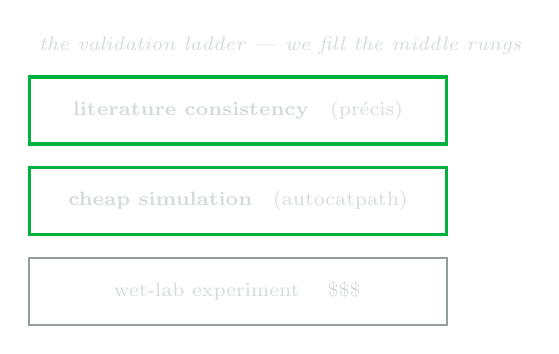
\begin{tikzpicture}[x=1cm,y=1cm,every node/.style={font=\scriptsize,text=LightText}]
        \draw[MutedGray,line width=0.8pt] (0,0) rectangle (5.3,0.85);
        \node at (2.65,0.425) {wet-lab experiment \quad \$\$\$};
        \draw[ULGreen,line width=1.2pt] (0,1.15) rectangle (5.3,2.0);
        \node at (2.65,1.575) {\textbf{cheap simulation} \; (autocatpath)};
        \draw[ULGreen,line width=1.2pt] (0,2.3) rectangle (5.3,3.15);
        \node at (2.65,2.725) {\textbf{literature consistency} \; (précis)};
        \node[anchor=west,font=\scriptsize\itshape] at (0,3.55) {the validation ladder --- we fill the middle rungs};
      \end{tikzpicture}
    \end{column}
  \end{columns}
\end{frame}

% ---------- 5 · thesis ----------
\begin{frame}{Our answer: ground the machine, budget the human}
  \citefield{}
  \centering
  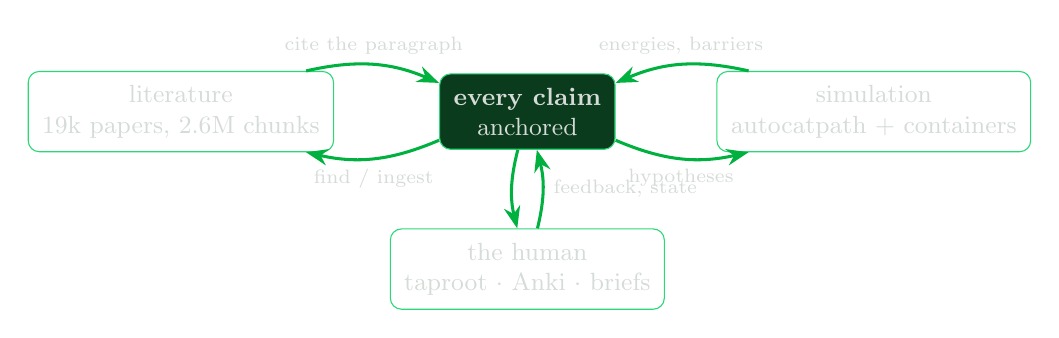
\begin{tikzpicture}[
      box/.style={draw=ULGreenBright,rounded corners,align=center,font=\small,inner sep=5pt,text=LightText},
      loop/.style={-{Stealth},ULGreen,line width=1.1pt},
      every node/.style={font=\small,text=LightText}]
    \node[box,fill=ULGreen!25!DarkBG] (claim) at (0,0) {\textbf{every claim}\\anchored};
    \node[box] (lit)  at (-4.4,0) {literature\\19k papers, 2.6M chunks};
    \node[box] (sim)  at (4.4,0)  {simulation\\autocatpath + containers};
    \node[box] (hum)  at (0,-2.0) {the human\\taproot \(\cdot\) Anki \(\cdot\) briefs};
    \draw[loop] (lit) to[bend left=18] node[above,font=\scriptsize]{cite the paragraph} (claim);
    \draw[loop] (claim) to[bend left=18] node[below,font=\scriptsize]{find / ingest} (lit);
    \draw[loop] (sim) to[bend right=18] node[above,font=\scriptsize]{energies, barriers} (claim);
    \draw[loop] (claim) to[bend right=18] node[below,font=\scriptsize]{hypotheses} (sim);
    \draw[loop] (claim) to[bend right=14] (hum);
    \draw[loop] (hum) to[bend right=14] node[right,font=\scriptsize]{feedback, state} (claim);
  \end{tikzpicture}

  \vspace{1ex}
  \small Both collaborators are \textbf{bounded-context agents}: the LLM has a token
  budget, the human has working memory and one screenful of sharp vision. Same
  discipline for both.
\end{frame}

% ---------- 5b · inside precis ----------
\begin{frame}{Inside précis: what the system holds}
  \citefield{live query, precis\_prod, 2026-08-13}
  \small
  \begin{itemize}\itemsep0.35ex
    \item[\sdone] One verb surface --- \texttt{get / search / put / edit /
          tag / link} --- over \textbf{54} kinds of thing (39 in active use).
          Everything below is those six verbs
    \item[\sdone] \textbf{Read:} papers (28{,}309 tracked, 19{,}651
          ingested), patents, news, web pages, email, encyclopedia entries,
          transcripts --- \textbf{2.6M} chunks, each summarized, keyworded,
          embedded, clustered
    \item[\sdone] \textbf{Written:} drafts, \LaTeX{} and markdown, figures,
          diagrams, slide decks, flashcards (7{,}264)
    \item[\sdone] \textbf{Modelled:} structures, proteins, materials,
          reaction routes and pathways --- and the hardware kinds: CAD, PCB,
          parts, datasheets
    \item[\sdone] \textbf{Given} to the agent: \textbf{143} skills ---
          ``how do I \ldots'', pulled at the moment of need --- plus the kind
          catalog and the model catalog
    \item[\sdone] \textbf{Grown} by the agent: \textbf{9{,}663} memories
          (9{,}222 of them dreamt), \textbf{49{,}403} typed links, 3{,}453
          agent logs --- the connections it found, not the ones we gave it
    \item[\sdone] \textbf{Self-ops:} todos (2{,}202 filed, 120 open),
          quests, jobs, alerts, gripes --- the system files its own bugs
  \end{itemize}
\end{frame}

% ---------- 6 · grounding in literature ----------
\begin{frame}{Grounding in literature}
  \citefield{live query, precis\_prod, 2026-08-13}
  \begin{itemize}
    \item[\sdone] Corpus: \textbf{19{,}651} papers fully ingested
          (28{,}309 tracked), \textbf{2.6M} searchable chunks, 101 patents
    \item[\sdone] One substrate: papers, patents, drafts, web pages, notes
          --- everything lands as \emph{chunks}, searchable by meaning,
          by string, by category, by link (next slide)
    \item[\sdone] Taproot: claim $\to$ supporting papers $\to$ \emph{the exact
          paragraph} (search-to-section)
    \item[\sdone] Citation-graph crawl keeps discovering and ingesting cited work
    \item[\srough] Argument graph: canonical claims with typed evidence
          across papers (establishes / corroborates / contradicts)
  \end{itemize}
\end{frame}

% ---------- 6a2 · one substrate ----------
\begin{frame}{One substrate, many ways in}
  \citefield{live query, precis\_prod, 2026-08-13}
  \begin{itemize}
    \item[\sdone] Papers, patents, drafts, web pages, notes, email ---
          everything lands as \emph{chunks} (2.6M); each gets a summary
          (token-efficient reading, for humans too), keywords, an
          embedding, and a cluster
    \item[\sdone] Ask by \emph{meaning}: semantic search over embeddings ---
          including the HyDE trick: draft the answer you \emph{wish}
          existed, embed it, find the passages that look like it
    \item[\sdone] Ask \emph{literally}: grep-style lexical and verbatim
          modes over the indexed full text
    \item[\sdone] Ask by \emph{category}: chunks are clustered for browsing
          and navigation; finer role / topic categorizers are layering in
    \item[\sdone] Ask by \emph{link}: walk the typed graph --- citations and
          evidence edges, down to the paragraph
    \item[\sdone] Heavily indexed for interactive speed: a \textbf{55\,GB}
          database, \textbf{24\,GB} of it indexes --- the vector store
          alone is 33\,GB. Approximate nearest-neighbour (ANN) indexing is what
          keeps it interactive: the closest of 2.6M embeddings without
          comparing against all of them
  \end{itemize}
\end{frame}

% ---------- 6a3 · finding the paper ----------
\begin{frame}{Finding the paper: the corpus hunts for itself}
  \citefield{src/precis/ingest/citations.py \(\cdot\) live stubs backlog}
  \begin{itemize}
    \item[\sdone] The citation graph does most of the finding: every read
          paper's reference list \emph{and} its citing papers (Semantic
          Scholar, both directions) become candidates
    \item[\sdone] Anyone can want a paper with one call --- a DOI mints a
          stub and the fetcher chases it: the human, a quest agent
          mid-argument, or a 3\,am dream
    \item[\sdone] Web and deep-research searches surface titles worth
          holding; title-only requests park in a backlog for triage
          instead of guessing a DOI
    \item[\sdone] Wanting is idempotent: re-requesting a held or already
          wanted paper is a no-op --- no duplicate hunts
    \item[\srough] Coverage watch: new corpus text probed against standing
          claims, so gaps announce themselves
  \end{itemize}
  \vspace{0.5ex}
  \centering
  {\scriptsize\color{MutedGray}\emph{Find them, get them, index them all.}}
\end{frame}

% ---------- 6b · paper acquisition ----------
\begin{frame}{Getting the paper: eleven ways, best version first}
  \citefield{src/precis/workers/fetch\_oa.py}
  \begin{itemize}
    \item[\sdone] An 11-leg cascade per paper: publisher APIs (Springer,
          Elsevier, Wiley) $\to$ open-access aggregators (Unpaywall,
          Crossref, OpenAlex, EuropePMC, CORE) $\to$ arXiv $\to$
          Semantic Scholar $\to$ paid content API \emph{last}
          ($\sim$1¢/file); the stubborn rest queue for \emph{assisted
          download} --- link ready, human clicks
    \item[\sdone] Version of record beats preprint; free beats paid ---
          the order of the legs \emph{is} the policy
    \item[\sdone] Markup first: publisher XML / JATS / arXiv \LaTeX{} source
          beat the PDF as the text source; PDF-only papers go through
          ML layout analysis + OCR (Marker) --- equations, tables and
          figures recovered as text, the PDF kept for printing only
    \item[\sdone] Retraction gate \emph{before} download --- retracted work
          never enters the corpus
    \item[\sdone] Retraction status is wired downstream too: retracted work
          is downranked in search and \emph{blocked} as a citation anchor at
          export --- a draft cannot ship citing a retracted paper
    \item[\sdone] Never gives up: retries back off to monthly ---
          ``a paper can become OA later''
    \item[\sdone] After fetch, the cascade: chunk $\to$ embed $\to$ summarize
          $\to$ extract keywords --- background worker passes; a paper arrives
          \emph{searchable}, no human in the loop
  \end{itemize}
\end{frame}

% ---------- 6c · paper checking ----------
\begin{frame}{Checking the paper: references, retractions, injections}
  \citefield{src/precis/workers/bib\_parse.py \(\cdot\) src/precis/utils/inject\_scan.py}
  \begin{itemize}
    \item[\sdone] Every held paper's bibliography is parsed: entries split,
          fields extracted (regex first, a small LLM for the stragglers),
          matched to a DOI --- and to our held copy when we have one
    \item[\sdone] Inline markers resolve: the \texttt{[12]} next to a number
          in the text answers ``which paper is that?'' in one call
    \item[\sdone] Provenance preflight: hand it a reference list, it flags
          retractions, amendments and metadata mismatches (Crossref)
    \item[\srough] ``List this paper's references'' for the agent: the table
          and the web view exist; the MCP verb is one view away
    \item[\sdone] Prompt-injection scan on everything fetched from outside
          (web, news, email): \emph{suspect} $\to$ bannered as untrusted,
          \emph{high} $\to$ body withheld. Deployed this week; the email
          model-scored tier is built but waits on mail polling. External
          text is delimited as data either way --- the scan is the alarm,
          not the protection
    \item[\sidea] Next: the same scan across ingested PDFs corpus-wide
  \end{itemize}
\end{frame}

% ---------- 7 · literature machinery ----------
\begin{frame}{Token-efficient literature machinery}
  \citefield{}
  \begin{columns}[T]
    \begin{column}{0.58\textwidth}
      \begin{itemize}
        \item[\sdone] Fisheye TOC: cluster-drill any paper; read paragraphs,
              not PDFs; pointer-sized handles (\texttt{pa203165\textasciitilde14..27})
        \item[\sdone] Discovery layer: per-chunk keywords + summaries,
              precomputed once, reused every query
        \item[\srough] Chunk-role categorizers (default-off cascade)
        \item[\sidea] Coverage audit: ``did we cite \emph{all} the relevant work?''
      \end{itemize}
    \end{column}
    \begin{column}{0.40\textwidth}
      \scriptsize
      {\color{LightText}%
      \begin{tabular}{@{}ll@{}}
        \toprule
        \multicolumn{2}{@{}l@{}}{\textbf{chunks} (excerpt)} \\
        \midrule
        \texttt{ref\_id, ord}      & position in paper \\
        \texttt{text, token\_count}& the paragraph \\
        \texttt{section\_path}     & where in the paper \\
        \texttt{page\_first/last}  & PDF anchor \\
        \texttt{keywords}          & discovery layer \\
        \texttt{handle}            & terse pointer \\
        \midrule
        \multicolumn{2}{@{}l@{}}{\textbf{links}: evidence edges, per-paragraph} \\
        \bottomrule
      \end{tabular}}
    \end{column}
  \end{columns}
\end{frame}

% ---------- 7a2 · fisheye sample ----------
\begin{frame}{Fisheye in practice: drill, don't read}
  \citefield{}
  \setlength{\fboxsep}{6pt}%
  \centering
  \fcolorbox{MutedGray}{DarkBG}{\begin{minipage}{0.94\textwidth}
    \scriptsize\ttfamily
    \textcolor{ULGreenBright}{get(id='pa47100\textasciitilde 17..18')}%
    ~~~\textcolor{MutedGray}{Cu-based SAAs for CO\(_2\) electroreduction $\cdot$ Angew.\ Chem.\ '26 $\cdot$ 144 chunks}\\[0.3ex]
    ~\textcolor{MutedGray}{\textasciitilde 15~~various cu-based saas $\cdot$ dopant-mediated mechanisms $\cdot$ c-c coupling}\\
    ~\textcolor{MutedGray}{\textasciitilde 16~~co2rr mechanisms $\cdot$ ai agent $\cdot$ targeted computational strategies}\\
    ~\textcolor{ULGreenBright}{\textasciitilde 17}~~``The energy descriptor demonstrates a linear correlation with the\\
    ~~~~~activation energy barriers of rate-determining step for C2+ formation''\\
    ~\textcolor{ULGreenBright}{\textasciitilde 18}~~``\ldots identifies the newly discovered M1/Cu(111) (M = Y, Lu) SAAs and\\
    ~~~~~Ni1Zn1/Cu, Rh1Zn1/Cu DSAAs as promising candidates with high C2+ selectivity''\\
    ~\textcolor{MutedGray}{\textasciitilde 19~~integrated workflow $\cdot$ three stages $\cdot$ universal design principle}\\[0.3ex]
    ~\textcolor{MutedGray}{path:}~\textcolor{ULGreenBright}{view='toc'}~\textcolor{MutedGray}{144 chunks $\to$ 3 clusters $\to$ \textasciitilde 15..20 $\to$ read 2 verbatim}
  \end{minipage}}

  \vspace{0.8ex}
  \begin{itemize}
    \item[\sdone] Sharp center, compressed periphery: the asked-for
          paragraphs verbatim, neighbors as one-line summaries ---
          context without the token bill. Under the hood it's a graph
          traversal over chunks and links --- assembled by code,
          zero LLM calls
    \item[\sdone] In-text citations resolve to \emph{held} papers ---
          one hop from a number to its source, for the LLM and the human
          alike
    \item[\sdone] Patents drill the same way (\texttt{kind='patent'}, 101 held)
    \item[\sidea] Next: resolved cites as one-line \emph{summaries}, not bare
          names --- judge a reference without opening it
  \end{itemize}
\end{frame}

% ---------- 7b · taproot claims (data model) ----------
\begin{frame}{Taproot: claims with receipts}
  \citefield{src/precis/taproot/}
  \begin{itemize}
    \item[\srough] A claim is a first-class object: one canonical sentence,
          citable by a short id --- identical claims \emph{converge} onto
          the same hub instead of duplicating
    \item[\srough] Support is multi-paper and paragraph-granular: evidence
          edges run paper $\to$ claim, one per supporting \emph{passage}
          --- two passages in one paper are two edges
    \item[\srough] Attaching evidence is a reading act: an LLM verifier
          accepts a passage only if it actually supports the claim;
          rejections are remembered, never re-billed
    \item[\sdone] Evidence must come from the \emph{meat} of the paper ---
          ``X was doped with Y and we measured Z'', not ``it is known
          that\ldots''. The hearsay gate now strikes references /
          prior-work / background sections and quotes carrying citation
          markers from the admissible pool (mint gate, next slides)
    \item[\sdone] Found the hard way: a claim whose support traced back to a
          review paragraph --- whose own sources did not support it.
          A review paragraph cites \emph{elsewhere}; accepting one as
          evidence launders an unchecked claim into a verified one
  \end{itemize}
\end{frame}

% ---------- 7b2 · taproot read side ----------
\begin{frame}{Taproot: trust at read time}
  \citefield{src/precis/taproot/ --- seniority.py}
  \begin{itemize}
    \item[\srough] How much to trust a claim is \emph{computed from its
          evidence each time you read it} --- never stored as a number that
          can go stale. Strongest to weakest: passage checked against the
          full paper, then abstract-only, then author-vouched, then
          unverified, then contradicted. Once verified against the full
          text it stays top-ranked: the paper \emph{was} read --- a later
          ``trust me'' can't unread it
    \item[\srough] Presented claim-first: the sentence up front, evidence
          on demand, and one jump lands \emph{in the right section of the
          paper} (deep search) --- no PDF, no scrolling. Cycle time is
          where the human loses focus, so the mechanical middle steps are
          eliminated
    \item[\srough] The same trust function feeds the editor badge and the
          .docx / \LaTeX{} exports --- one truth, three surfaces
  \end{itemize}
\end{frame}

% ---------- 7c · argument graph ----------
\begin{frame}{The argument graph}
  \citefield{src/precis/taproot/ --- hub.py, seniority.py}
  \begin{itemize}
    \item[\srough] Typed edges: establishes / corroborates / contradicts
          (paper $\to$ claim); refines / contradicts (claim $\leftrightarrow$
          claim)
    \item[\srough] Originators are derived, never guessed: citation edges
          \emph{among the supporters} decide who was first; no evidence,
          no originator --- just an honest coverage note
    \item[\srough] Over-merge is the one forbidden direction: unconfirmed
          matches go to human review, and the live gate requires
          \emph{zero} false merges
    \item[\srough] Coverage watch --- ``did we cite all the relevant
          work?'': every newly embedded paragraph is probed against every
          claim; near-misses queue for evidence review
    \item[\sdone] Status: producers live --- 1,552 canonical claim hubs,
          2,059 evidence edges in prod, and the publication surface on top
          (next two slides)
  \end{itemize}
\end{frame}

% ---------- 7d · nanopublications ----------
\begin{frame}{Nanopublications: claims signed to the world}
  \citefield{src/precis/nanopub/ --- mint.py, keys.py, ots.py, registry.py}
  \begin{itemize}
    \item[\sdone] A claim hub that survives the gates becomes a
          \emph{nanopublication}: one sentence + provenance + grounding
          (DOI, PDF hash, verbatim quote) as a tiny signed artifact ---
          verifiable \emph{offline} by a third party, no server of ours up
    \item[\sdone] The ladder ratchets frozen-ness: candidate $\to$ reviewed
          (string freezes) $\to$ signed (bytes freeze) $\to$ anchored
          (OpenTimestamps, Bitcoin calendar) $\to$ published (public
          forever) --- every rung before publish is reversible
    \item[\sdone] Two keys, two meanings: the bot key is non-attesting;
          the human attesting key loads only through an interactive door
          and must match the signer's registered ORCID iD ---
          ``signed'' means \emph{a person checked}
    \item[\sdone] New contradicting evidence walks the ladder \emph{down}:
          a reviewed or signed claim reopens to candidate; past the
          anchor, a human must supersede or retract
    \item[\sdone] Live since 2026-08-24: first claim published to the
          public nanopub registry (w3id.org trusty URI, OTS-anchored);
          3 more signed, 138 candidates queued behind the human doors
    \item[\sdone] Mirror of everyone else: $\sim$89k published nanopubs
          from the global registry cached + hash-verified locally, with a
          concurrence alert when someone else asserts one of our sentences
  \end{itemize}
\end{frame}

% ---------- 7e · the claim gates ----------
\begin{frame}{The claim gates: what a sentence survives to go public}
  \citefield{src/precis/nanopub/gates.py, preflight.py \(\cdot\) src/precis/taproot/}
  \small
  \begin{itemize}\itemsep0.25ex
    \item[\sdone] \textbf{Admission}: only papers, patents, EDGAR filings
          and datasheets ground evidence --- a draft or memory never can;
          the passage must be asserting prose; an LLM verifier accepts it
          only if it supports the claim; a dialectic argument without an
          inline evidence handle never enters the record
    \item[\sdone] \textbf{Placement}: a sub-confidence duplicate goes to
          human review, never auto-merges (live eval: \emph{zero} false
          merges); \emph{contradicts} is written only at high confidence
          --- it blocks someone's publication
    \item[\sdone] \textbf{Mint} --- mechanical validators, no LLM in the
          path: verbatim quote in exactly one stored chunk $\cdot$ unique
          search snip $\cdot$ DOI + PDF hash $\cdot$ hearsay struck
          (reference / prior-work sections, quotes with citation markers,
          review-titled sources, papers we don't hold) $\cdot$ quantity
          bounds $\cdot$ fields contained in quotes $\cdot$ authoring
          model named $\cdot$ live \emph{contradicts} blocks $\cdot$
          drift (sentence re-hashed) $\cdot$ atoms sign before compounds
    \item[\sdone] \textbf{Type discipline}: a claim without a quote is
          blocked --- a hypothesis \emph{with} one is blocked too: it
          carries motivation + a discriminating experiment
          ($\geq$2 independent source papers), never evidence
    \item[\sdone] \textbf{Publish preflight} --- no mute button: every
          evidence edge machine-verified against the \emph{live} sentence
          or human-signed-off interactively; trust allowlist --- a bot
          signature alone publishes nothing; the POST is interactive +
          live-flagged + zero blocking issues
    \item[\sidea] Still judgment, not code: commensurability of a
          compound's binding; adjudicating a reopened dispute; retraction
          past the anchor
  \end{itemize}
\end{frame}

% ---------- 8 · autocatpath: the algorithm ----------
\begin{frame}{autocatpath I: auto-generating the reaction network}
  \citefield{\href{https://github.com/retospect/catpath}{github.com/retospect/catpath} --- explore.py}
  \centering
  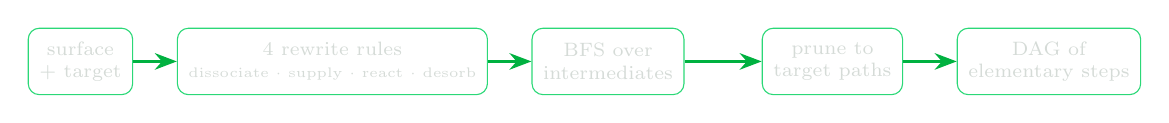
\begin{tikzpicture}[
      stage/.style={draw=ULGreenBright,rounded corners,align=center,
                    font=\scriptsize,inner sep=4pt,text=LightText,minimum height=2.4em},
      go/.style={-{Stealth},ULGreen,line width=1.1pt}]
    \node[stage] (in)    at (0,0)    {surface\\+ target};
    \node[stage] (rules) at (3.2,0)  {4 rewrite rules\\{\tiny dissociate \(\cdot\) supply \(\cdot\) react \(\cdot\) desorb}};
    \node[stage] (bfs)   at (6.7,0)  {BFS over\\intermediates};
    \node[stage] (prune) at (9.55,0) {prune to\\target paths};
    \node[stage] (dag)   at (12.3,0) {DAG of\\elementary steps};
    \draw[go] (in) -- (rules); \draw[go] (rules) -- (bfs);
    \draw[go] (bfs) -- (prune); \draw[go] (prune) -- (dag);
  \end{tikzpicture}

  \vspace{1ex}
  \begin{itemize}
    \item[\sdone] Species are molecular \emph{graphs} on the surface; four
          rewrite rules generate every elementary step: break a bond, stage
          an adatom (+H*/+O*), bond it, or let a closed-shell fragment leave
    \item[\sdone] Intermediates found by breadth-first search with canonical-graph
          dedup, valence and atom-budget caps --- every step strictly makes
          progress, so the network is provably a DAG
    \item[\sdone] Geometries materialised per intermediate with a shared atom
          ordering across each step --- exactly what NEB interpolation needs
    \item[\sdone] Curated templates remain available when the chemistry is known
  \end{itemize}
\end{frame}

% ---------- 8b · autocatpath: scoring ----------
\begin{frame}{autocatpath II: spend barriers only where they matter}
  \citefield{\href{https://github.com/retospect/catpath}{github.com/retospect/catpath} --- pipeline.py, neb.py}
  \begin{itemize}
    \item[\sdone] Relax every intermediate (BFGS, force + energy
          convergence) with ML potentials; barriers by climbing-image NEB
          on IDPP-interpolated bands, auto-retried on non-convergence;
          coadsorbed fragments by default
    \item[\sdone] Routes ranked by \emph{energetic span} (Kozuch--Shaik);
          unrefined steps count as optimistic lower bounds, so ranking works
          before every barrier exists
    \item[\sdone] Best-first NEB scheduling: refine only the step that could
          change the winning route; stop when no rival route can win ---
          barriers are bought, not sprayed
    \item[\sdone] \textbf{Dissolving tether}: each adsorbate atom on a spring to
          the slab, stiffness ramped to zero across relaxations --- strays are
          pulled back into the well, yet every reported number is spring-free
    \item[\sdone] Uncertainty pooled across seeds \emph{and} potentials
          (MACE / CHGNet / UMA / GRACE); CHE post-processing gives limiting +
          operating potential (V vs RHE)
  \end{itemize}
\end{frame}

% ---------- 8b2 · autocatpath: the vocabulary ----------
\begin{frame}{autocatpath, decoded}
  \citefield{}
  \small
  {\color{LightText}%
  \begin{tabular}{@{}p{0.24\textwidth}p{0.70\textwidth}@{}}
    \toprule
    \textbf{ML potential} & a neural net trained to reproduce quantum-chemistry
      (DFT) energies and forces --- orders of magnitude cheaper, slightly
      wrong; we run \emph{four} and let their disagreement be the error bar \\
    MACE $\cdot$ CHGNet $\cdot$ UMA $\cdot$ GRACE & the four: independent
      architectures and training sets, so their errors don't correlate \\
    \textbf{(CI-)NEB} & nudged elastic band: stretch a chain of geometries
      between two states and relax it; the \emph{climbing image} slides to
      the saddle point --- that saddle \emph{is} the barrier \\
    \textbf{CHE} & computational hydrogen electrode: every
      $\mathrm{H^+{+}e^-}$ step shifts by $-eU$ --- potential dependence
      without simulating an electrode \\
    \textbf{energetic span} & the one effective barrier of the whole cycle
      (Kozuch--Shaik) --- what actually limits the rate, not the tallest
      single step \\
    $U_L$ (V vs RHE) & limiting potential: the least negative potential at
      which every step runs downhill; quoted against the reversible
      hydrogen electrode \\
    \bottomrule
  \end{tabular}}
\end{frame}

% ---------- 8c · autocatpath: outputs ----------
\begin{frame}{autocatpath III: three audiences, three outputs}
  \citefield{src/precis\_pathway/}
  \begin{itemize}
    \item[\sdone] \textbf{For the human}: a self-contained offline HTML report
          --- clickable energy profile linked to rotatable 3-D structures,
          gallery, collapsible methods
    \item[\sdone] \textbf{For the workbench}: results land as an interactive
          \texttt{pathway} ref in précis --- DAG, profiles, cross-model
          compare, dossiers, U-slider
    \item[\sdone] \textbf{For the quest loop}: a scalar summary
          (rate-limiting barrier, span, $U_L$, selectivity / trap / poison
          margins) harvested automatically as quest measures
    \item[\sdone] Every run: \texttt{methods.md} + a provenance snapshot ---
          the write-up paragraph is generated, not reconstructed
  \end{itemize}
\end{frame}

% ---------- 9 · wider sim substrate + LLM hands ----------
\begin{frame}{Beyond one code: the simulation substrate}
  \citefield{}
  \begin{itemize}
    \item[\sdone] Pathway explorer UI + dossiers inside précis
          (tier ladder, potential lever, lineage/dedup)
    \item[\srough] Open catalysis DBs imported locally (OC20 vs AQCat25
          pick pending)
    \item[\srough] Python simulation containers (sandbox-run; built, dark)
    \item[\sidea] CFD and CAD-for-CFD geometry via a cascade of simulators
          matched to each order of magnitude
    \item[\sidea] National HPC (ICHEC) as the big-compute rung: ML-potential
          sweeps and DFT where the local boxes stop
  \end{itemize}
\end{frame}

% ---------- 9c · LLM hands on the model ----------
\begin{frame}{LLM hands on the model}
  \citefield{src/precis/handlers/structure.py}
  \begin{columns}[T]
    \begin{column}{0.55\textwidth}
      \begin{itemize}
        \item[\sdone] Whole simulations by run spec: edit the spec $\to$ run
              $\to$ profile / DAG / thumbnails come back
        \item[\sdone] A slab is a \emph{typed design}: the LLM authors ops
              and reads probes, never pixels --- pattern proven on the CAD
              and PCB kinds first
        \item[\sdone] Semantic diff: edit, then ask what changed --- bonds
              formed / broken, atoms displaced --- modify the model,
              \emph{see what it did}
        \item[\sdone] Guardrails: impossible geometry hard-rejected before
              any GPU spend; cheap local relax first, cloud last resort
        \item[\srough] Designs cite their reasons: the structure assembles
              its own literature query; provenance links say \emph{why}
              it exists
      \end{itemize}
    \end{column}
    \begin{column}{0.42\textwidth}
      \scriptsize
      {\color{LightText}%
      \begin{tabular}{@{}l@{}}
        \toprule
        \textbf{navigate / inspect} \\
        \midrule
        \texttt{get(view='neighborhood'|'bonds'|'find')} \\
        \texttt{get(view='plane'|'rings'|'path'|'pov')} \\
        \texttt{get(view='diff')} ~~ what changed \\
        \texttt{get(view='validate')} ~~ is it physical \\
        \texttt{get(view='literature')} ~~ why it exists \\
        \texttt{get(view='poscar'|'cif'|'extxyz')} \\
        \bottomrule
      \end{tabular}}

      \vspace{1ex}
      {\color{LightText}%
      \begin{tabular}{@{}l@{}}
        \toprule
        \textbf{write: \texttt{edit(ops=[...])}} \\
        \midrule
        \texttt{slab} ~~ seed a whole fcc(111) surface \\
        \texttt{add\_atom $\cdot$ set\_element $\cdot$ vacancy} \\
        \texttt{displace $\cdot$ add\_bond $\cdot$ remove\_bond} \\
        \texttt{constrain $\cdot$ eye $\cdot$ measure} \\
        \bottomrule
      \end{tabular}}

      \vspace{0.6ex}
      \tiny\textcolor{MutedGray}{\texttt{slab} mirrors autocatpath's
      \texttt{build\_slab} --- identical atom order, so a design injects
      straight into a barrier run.}
    \end{column}
  \end{columns}
\end{frame}

% ---------- 9b · corpus to manuscript ----------
\begin{frame}{From corpus to manuscript}
  \citefield{src/precis/export/endnote.py}
  \begin{itemize}
    \item[\sdone] Chunk-native drafts: every paragraph keeps its evidence
          links as it is written and rewritten
    \item[\sdone] Citations generated from taproot: one call per source
          $\to$ BibTeX / RIS / EndNote
    \item[\sdone] .docx export embeds an EndNote \emph{traveling library}
          (reverse-engineered Cite-While-You-Write fields) --- co-authors
          open Word and the references are simply there
    \item[\sdone] Figures extracted at ingest with page anchors --- image
          sources are cited like text
    \item[\sdone] Third-party figures tracked by rights: origin
          (original / own graph / third-party) + permission with expiry
          --- an uncleared figure \emph{fails the export}, like a bare
          cite fails review
    \item[\sdone] A draft citing a signed claim gets a ``Published claim
          artifacts'' appendix --- frozen sentence + trusty URI --- in
          both exporters; unminted claims leave the export byte-identical
    \item[\sidea] Living outputs: this deck and the paper, regenerated as
          the corpus moves
  \end{itemize}
\end{frame}

% ---------- 10 · human loop I ----------
\begin{frame}{Grounding the human I: the other context window}
  \citefield{}
  \begin{itemize}
    \item Human working memory is the scarce resource: recall is slow,
          screens are small --- optimize for it like we optimize tokens
    \item The fovea --- the only sharp patch of the retina --- covers a word
          or two at reading distance, far \emph{smaller than the screen};
          ``seeing the page'' is a behavioral trick of constant eye jumps.
          Design for the sharp spot, not for the page
    \item[\sdone] Taproot presentation: claim first, evidence on demand,
          jump straight to the section
    \item[\sdone] Terse pointer handles keep human--machine exchanges short
          on both sides
    \item[\srough] Turn-taking: the system paces itself instead of flooding
          the channel
  \end{itemize}
\end{frame}

% ---------- 11 · human loop II ----------
\begin{frame}{Grounding the human II: sensing and shaping}
  \citefield{}
  \begin{itemize}
    \item Experts recall vast latent detail in a blink; elsewhere the same
          person's understanding is sparse --- and telling which is which
          is genuinely hard, from outside \emph{and} inside
    \item[\srough] Anki integration: the system's running estimate of what
          the human actually retains --- sensing the human is hard, and
          that is exactly why it matters
    \item[\sdone] Morning / evening briefs: podcast \emph{and} text ---
          listen on the commute, grep it back out later
    \item[\sidea] Weekly / monthly digests of newly ingested work
    \item[\sidea] The perpetually managed paper: semi-annual updates,
          always current --- this deck is its seed
  \end{itemize}
\end{frame}

% ---------- 12 · orchestration ----------
\begin{frame}{Untiring: the researcher loop, run all night}
  \citefield{}
  \centering
  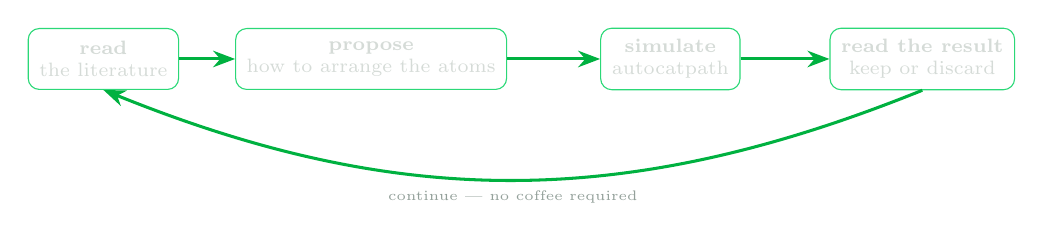
\begin{tikzpicture}[
      stg/.style={draw=ULGreenBright,rounded corners,align=center,
                   font=\scriptsize,inner sep=4pt,text=LightText,minimum height=2.2em},
      go/.style={-{Stealth},ULGreen,line width=1.1pt}]
    \node[stg] (read) at (0,0)   {\textbf{read}\\the literature};
    \node[stg] (prop) at (3.4,0) {\textbf{propose}\\how to arrange the atoms};
    \node[stg] (sim)  at (7.2,0) {\textbf{simulate}\\autocatpath};
    \node[stg] (res)  at (10.4,0){\textbf{read the result}\\keep or discard};
    \draw[go] (read) -- (prop);
    \draw[go] (prop) -- (sim);
    \draw[go] (sim) -- (res);
    \draw[go] (res.south) to[bend left=22]
      node[below,font=\tiny,text=MutedGray]{continue --- no coffee required} (read.south);
  \end{tikzpicture}

  \vspace{1ex}
  \begin{itemize}
    \item[\srough] What a researcher does --- but it doesn't stop at 6pm:
          quests keep the loop turning overnight
    \item[\srough] Honestly: \emph{autonomous exploration} is the flaky
          part --- it still fails a lot. Everything around it is
          surprisingly stable, and failures are usually one Claude
          session away from fixed
          \textcolor{MutedGray}{\emph{(the Shannon does flow past UL)}}
    \item[\sdone] Work \emph{parks itself} on a missing paper or pending
          feedback and resumes alone when it arrives
    \item[\sdone] Review tiers (nursery $\to$ structural $\to$ deep) gate
          what sticks; anti-spin guards + budget breaker bound the night
    \item[\sdone] Dreaming pass: far-apart points in embedding space,
          connected through a scientific lens --- inspiration, never citation
  \end{itemize}
\end{frame}

% ---------- 12a2 · dreaming ----------
\begin{frame}{Dreaming: speculative connections on idle compute}
  \citefield{src/precis/data/prompts/dream-prompt.md \(\cdot\) live memory me205091, 2026-08-13}
  \setlength{\fboxsep}{5pt}%
  \centering
  {\scriptsize
  \fcolorbox{MutedGray}{DarkBG}{\begin{minipage}{0.94\textwidth}
    \ttfamily
    \textcolor{MutedGray}{DREAM CYCLE --- no user is reading. Fact-anchored
    speculative connections, not introspection.}\\
    \textcolor{ULGreenBright}{1}~sample your \emph{own old memories} ---
    diverse, not recent (view='dreamable')\\
    \textcolor{ULGreenBright}{2}~sample papers the same way; pick one you
    don't recognise and read it\\
    \textcolor{ULGreenBright}{3}~pull one anchor from another kind:
    patent \(\cdot\) oracle \(\cdot\) web \(\cdot\) deep research\\
    \textcolor{ULGreenBright}{4}~write \(\geq\)2 non-obvious cross-kind
    connections --- each must pass through a fact\\
    \textcolor{ULGreenBright}{5}~request papers you wish you had
    (stubs are chased and auto-fetched later)\\
    \textcolor{ULGreenBright}{6}~verify your own work: every cited handle
    must resolve; promote survivors, keep failed hunches \emph{as hunches}
  \end{minipage}}\\[0.8ex]
  \fcolorbox{ULGreen}{DarkBG}{\begin{minipage}{0.94\textwidth}
    \textcolor{ULGreenBright}{\ttfamily me205091 \(\cdot\)
    tier:synthetic-insight}~\textcolor{MutedGray}{(survived its own review)}\\[0.2ex]
    ``NrfA wins its six-electron nitrite\(\to\)NH\(_3\) selectivity by
    \emph{compartmentalising delivery}, not by tuning an exposed site:
    the substrate binds in a secluded pocket on a lysine-ligated heme, with
    four further hemes wired in as an electron relay
    \textcolor{ULGreenBright}{[pa202554, pa3039]}. That is the solved,
    biological form of the critique my own earlier memories aimed at the
    quest's Pd-slab Pareto --- the rate limit is local proton and electron
    \emph{supply} to a buried site, not the intrinsic barrier of a bare slab.
    It argues for the confined-water / proton-shuttle overlayer as the
    synthetic analogue.''
  \end{minipage}}}

  \vspace{0.5ex}
  \begin{itemize}
    \item[\sdone] Runs on idle local compute, $\sim$every 15 minutes ---
          \textbf{9{,}222} dream memories so far
    \item[\sdone] One anchor seeded from an active quest, the other
          free-roams --- cross-domain by construction (paper
          \(\leftrightarrow\) patent \(\leftrightarrow\) web)
    \item[\sdone] Every dream adds edges: the link graph densifies, so
          tomorrow's search finds paths today's couldn't
  \end{itemize}
\end{frame}

% ---------- 12a3 · llm vs code ----------
\begin{frame}{Division of labor: what the LLM does, what code does}
  \citefield{}
  \begin{itemize}
    \item[\sdone] \textbf{The LLM as scientist} --- judgment work: reads
          papers, forms hypotheses, decides how to arrange the atoms,
          weighs what the simulation returned
    \item[\sdone] \textbf{The LLM as coder} --- builds the system itself,
          at build time: gated by tests, one worktree per session
          (the dev-loop slides)
    \item[\sdone] \textbf{Code serving the LLM} --- at runtime,
          deterministic machinery does the heavy lifting: fisheye context
          assembly (a graph traversal), search + ranking, autocatpath's
          path search and barrier pipeline, the worker cascade ---
          cheap, reproducible, zero tokens
    \item[\sdone] The rule of thumb: what must be \emph{right every time}
          becomes code; what needs \emph{judgment} stays with the LLM
    \item[\srough] The boundary migrates: a transformation the LLM finds
          itself doing twice gets written down as code the third time
  \end{itemize}
\end{frame}

% ---------- 12b · tool surface ----------
\begin{frame}{A deliberately small tool surface}
  \citefield{README --- ``one tool surface, seven verbs''}
  \begin{columns}[T]
    \begin{column}{0.52\textwidth}
      \begin{itemize}
        \item[\sdone] Seven verbs, one \texttt{kind=} discriminator ---
              the entire MCP surface an agent ever sees
        \item[\sdone] Skills are \emph{embedded}: agents discover the
              manual semantically (\texttt{search(kind='skill',
              q=goal)}) instead of having it stuffed into every prompt
        \item[\sdone] Small surface $=$ small schemas $=$ tokens saved
              on \emph{every single} tool call
      \end{itemize}
    \end{column}
    \begin{column}{0.44\textwidth}
      \scriptsize
      {\color{LightText}%
      \begin{tabular}{@{}ll@{}}
        \toprule
        \multicolumn{2}{@{}l@{}}{\textbf{the whole API}} \\
        \midrule
        \texttt{search} & find --- lexical $+$ semantic \\
        \texttt{get}    & read a ref, or compute \\
        \texttt{put}    & create / import / annotate \\
        \texttt{edit}   & anchored region edits \\
        \texttt{delete} & remove (recoverable) \\
        \texttt{tag}    & classify along typed axes \\
        \texttt{link}   & typed relations between refs \\
        \midrule
        \multicolumn{2}{@{}l@{}}{$\times$~\texttt{kind=} paper, patent, draft, quest,} \\
        \multicolumn{2}{@{}l@{}}{\phantom{$\times$~}cad, pcb, protein, email, \ldots{} (53)} \\
        \bottomrule
      \end{tabular}}
    \end{column}
  \end{columns}
\end{frame}

% ---------- 12bb · the database ----------
\begin{frame}{One ACID database under everything}
  \citefield{PostgreSQL + pgvector --- 121 forward-only migrations}
  \begin{columns}[T]
    \begin{column}{0.58\textwidth}
      \begin{itemize}
        \item[\sdone] Everything is a ref in PostgreSQL: papers, claims,
              quests, jobs, gripes --- \textbf{78} tables, one
              transactional truth
        \item[\sdone] ACID is what makes \emph{many agents} safe: atomic
              ingest, advisory-lock claims, lease tables --- relations
              never clobbered, work never done twice
        \item[\sdone] Append-only where it matters: body chunks are never
              mutated; migrations are forward-only
        \item[\sdone] Vectors live beside the rows (pgvector) --- no
              second database to drift out of sync
        \item[\srough] Multi-user by construction: role-separated access
              through a pooler --- scales to a small team without
              redesign
      \end{itemize}
    \end{column}
    \begin{column}{0.38\textwidth}
      \scriptsize
      {\color{LightText}%
      \begin{tabular}{@{}ll@{}}
        \toprule
        \multicolumn{2}{@{}l@{}}{\textbf{key tables}} \\
        \midrule
        \texttt{refs}             & every object \\
        \texttt{chunks}           & 2.6M paragraphs \\
        \texttt{chunk\_embeddings}& the vectors \\
        \texttt{links}            & typed relations \\
        \texttt{ref\_tags}        & status / axes \\
        \texttt{jobs}             & the factory ledger \\
        \texttt{ref\_events}      & full audit trail \\
        \bottomrule
      \end{tabular}}
    \end{column}
  \end{columns}
\end{frame}

% ---------- 12c · LLM router ----------
\begin{frame}{One router, every model}
  \citefield{\href{https://www.ichec.ie/academic/national-hpc}{ichec.ie --- Irish national HPC}}
  \begin{itemize}
    \item[\srough] Capability-tiered routing: each call states what it
          needs; the router picks the cheapest model that clears the bar
    \item[\srough] Chains: local-first with cloud fallback per tier; an
          \texttt{llm} catalog kind tracks variant-precise offerings
    \item[\srough] Proprietary content pinned to local models ---
          sovereignty enforced as a routing rule, not a promise
    \item[\srough] Status: built end-to-end --- awaits its first full
          deploy and a debugging pass
    \item[\srough] National-HPC burst: biggest local models via Slurm on
          ICHEC (built, dark --- awaiting cluster access)
    \item[\sidea] Provider cascade: local $\to$ OpenRouter $\to$ Anthropic
          with automatic failover
  \end{itemize}
\end{frame}

% ---------- 13 · own silicon ----------
\begin{frame}{Runs on our own silicon}
  \citefield{}
  \begin{itemize}
    \item[\sdone] A small office fleet --- a few Macs and a pair of DGX
          Sparks sharing one NAS --- is the factory floor
    \item[\sdone] Large open-weight models served in-house carry the bulk
          of the load; cloud only where capability demands it
    \item[\srough] Economics instrumentation: tokens per answered question,
          \$/day local vs cloud (probe in flight)
  \end{itemize}
  \vspace{0.5ex}
  \centering\small\textcolor{ULGreenBright}{\textbf{Grounded \emph{and} cheap enough to
  run all night --- that is the pitch.}}\\
  \small\textcolor{MutedGray}{\emph{(There is more compute at home than in the entire lab.)}}
\end{frame}

% ---------- 14 · evaluation ----------
\begin{frame}{Evaluation: how we will know it works (proposed)}
  \citefield{}
  \begin{itemize}
    \item[\sdone] Today: every artifact still gets a manual end-to-end
          review before it leaves the building --- \emph{no slop ships};
          the metrics below complement that, they don't replace it
    \item[\sidea] Citation integrity: \% of claims whose anchor resolves,
          + spot-audit ``does the paragraph actually support the claim''
    \item[\sidea] Coverage: recall against must-cite sets built from review
          articles' bibliographies
    \item[\srough] Simulation: autocatpath vs published barriers / limiting
          potentials on known systems; cross-potential agreement already a
          built-in error bar
    \item[\sidea] Cost: tokens per \emph{grounded} claim, vs plain RAG
    \item[\sidea] Human loop: Anki retention as the measurable of the
          human-side pipeline
  \end{itemize}
\end{frame}

% ---------- 15 · dogfooding ----------
\begin{frame}{Dogfooding: the system reports on itself}
  \citefield{}
  \begin{itemize}
    \item[\sdone] This deck's numbers were pulled live from the production
          database; the dots reflect actual deploy state
    \item[\sdone] The system files gripes on itself --- \textbf{391} filed,
          \textbf{275} in the last 30 days --- 242 of those already closed,
          \textbf{29} still open; agent-transcript
          mining turns LLM confusion into documentation fixes
    \item[\sidea] The paper will be a living précis draft --- the artifact
          demonstrates the method
  \end{itemize}
\end{frame}

% ---------- 15b · two manuals I ----------
\begin{frame}{Two manuals I: skills for the research agents}
  \citefield{src/precis/data/skills/ --- 143 skills}
  \begin{itemize}
    \item[\sdone] The product's manual lives \emph{in} the product:
          \textbf{143} skills served as refs --- the agent literally asks
          \texttt{search(kind='skill', q='how do I \ldots')} at the
          moment of need
    \item[\sdone] Token economy: nothing preloaded --- a session carries
          only the recipes it actually pulled, not a 143-chapter manual
          in every prompt
    \item[\sdone] They teach research conduct: how to cite, how to attach
          evidence, per-kind recipes, whole tool-call sequences
          (toolpaths)
    \item[\sdone] Self-improving: transcript mining turns agent confusion
          into skill fixes; gripes point at the gaps
    \item[\sdone] The agents read the same manual they help improve
  \end{itemize}
\end{frame}

% ---------- 15c · two manuals II ----------
\begin{frame}{Two manuals II: skills for the coder}
  \citefield{CLAUDE.md \(\cdot\) AGENTS.md \(\cdot\) docs/}
  \begin{itemize}
    \item[\sdone] The repo carries a \emph{separate} manual for the agents
          that build précis: ship workflow (\texttt{/land}, \texttt{/go}),
          test discipline, backlog care, conventions-that-bite
    \item[\sdone] Kept deliberately apart: ``how to cite'' and ``how to
          land a branch'' confound easily --- different readers, different
          manuals, never mixed
    \item[\sdone] One source of truth per fact: codebase map $\to$ package
          docstrings $\to$ glossary; generated indexes, never hand-edited
    \item[\sdone] 19 sized agent roles (cheap gophers $\to$ deep
          reviewers) --- delegation is the cost lever
    \item[\sdone] Memory that survives context compaction: threads,
          runbooks, gotchas --- the coder wakes up knowing what bit it
          last time
  \end{itemize}
\end{frame}

% ---------- 16 · N=1 to lab ----------
\begin{frame}{From N=1 to a lab}
  \citefield{}
  \begin{itemize}
    \item[\sdone] Already multi-agent with one shared, provenance-carrying
          corpus --- adding humans scales the readers, not the truth
    \item[\sidea] Per-member human loop: own Anki state, own briefs, own
          reading queue over the shared substrate
    \item[\sidea] Specialization by quest: members own quests, agents
          specialize per quest --- \textbf{shared knowledge stays in the
          argument graph and term registry}, so expertise diverges without
          the ontology forking
    \item[\sidea] Onboarding: taproot + the brief backlog --- catch up in
          weeks, not a year of reading
  \end{itemize}
\end{frame}

% ---------- 16a0 · inside claude code ----------
\begin{frame}{Inside Claude Code: the harness that writes it}
  \citefield{.claude/ \(\cdot\) scripts/hooks/ --- repo configuration}
  \small
  \begin{itemize}\itemsep0.35ex
    \item[\sdone] \textbf{Given} to the coder: \textbf{19} sized agent roles
          (8 mechanical, 11 for bounded changes; architecture stays with the
          main loop), 6 one-word workflows (\texttt{/land}, \texttt{/go},
          \texttt{/next}\ldots), \textbf{61} scripts
    \item[\sdone] \textbf{Enforced, not requested:} \textbf{20} hooks fire
          \emph{inside} the agent's tool calls at 5 lifecycle points ---
          blocking writes to production, edits to sealed migrations, commits
          on \texttt{main}, secret reads, blind \texttt{git stash}
    \item[\sdone] The softer ones redirect instead of blocking: a
          bare-symbol grep becomes a structural query; a stale map or an
          unexplained bug triggers the triage path
    \item[\sdone] \textbf{Grown} by the coder: \textbf{93} memory files ---
          threads, runbooks, gotchas --- reloaded every session, so it wakes
          up knowing what bit it last time
    \item[\sdone] \textbf{Written down:} 12 conventions, 16 runbooks,
          \textbf{198} open backlog items, and one router document that
          points at the rest
    \item[\sdone] Same shape as précis itself: a manual and tools handed
          over, memory and links accumulated --- the symmetry is deliberate
  \end{itemize}
\end{frame}

% ---------- 16a · the dev loop ----------
\begin{frame}{The dev loop behind the curve}
  \citefield{AGENTS.md \(\cdot\) scripts/ship}
  \begin{itemize}
    \item[\sdone] Shipping is one word: \texttt{/land} = commit $\to$ sync
          $\to$ containerized gate (ruff, mypy, tests) $\to$ squash to
          main; \texttt{/go} adds the full suite + cluster deploy
    \item[\sdone] Branching: trunk-based --- one short-lived branch per
          session worktree, squashed onto an always-green \texttt{main}
          (one commit per ship, linear history); no develop or release
          branches, a branch dies when it lands
    \item[\sdone] Many Claude sessions in parallel worktrees; merges are
          lock-free compare-and-swap pushes; finished worktrees reap
          themselves
    \item[\sdone] Inner loop runs only the tests the change touches
          (testmon); the full suite gates every deploy
    \item[\sdone] Backlog: one file per item (\textbf{198} open), deleted
          on ship --- git log is the only done-log; gripes catch the
          residuals
    \item[\sdone] The dev context is budgeted like tokens: CLI output
          compressed 60--90\%, semantic code index, memory that survives
          compaction
  \end{itemize}
\end{frame}

% ---------- 16a2 · LLM coding experience ----------
\begin{frame}{Coding with an LLM: where the human time goes}
  \citefield{experience report --- 1{,}989 commits, 22 weeks}
  \begin{itemize}
    \item[\sdone] Almost no time reviewing code line-by-line --- attention
          goes to \emph{data structures}: tables, schemas, invariants,
          interfaces. Get those right and the generated code follows
    \item[\sdone] Hardly any object-oriented design to argue about either ---
          the codebase converged on plain data + functions, a shape the
          model handles very well
    \item[\sdone] Stability comes from the harness, not from trust: lint,
          typecheck and unit tests gate every merge; red never ships
    \item[\sdone] The recurring failure mode is small: occasional web-UI
          JavaScript glitches --- paste the browser console into the
          session, fixed in 1--2 turns
    \item[\sdone] Net: \emph{very} stable. Five months of daily LLM-written
          commits and the system stays up
  \end{itemize}
\end{frame}

% ---------- 16b · effort ----------
\begin{frame}{Five months of effort}
  \citefield{git log, precis-mcp, 2026-08-13}
  \centering
  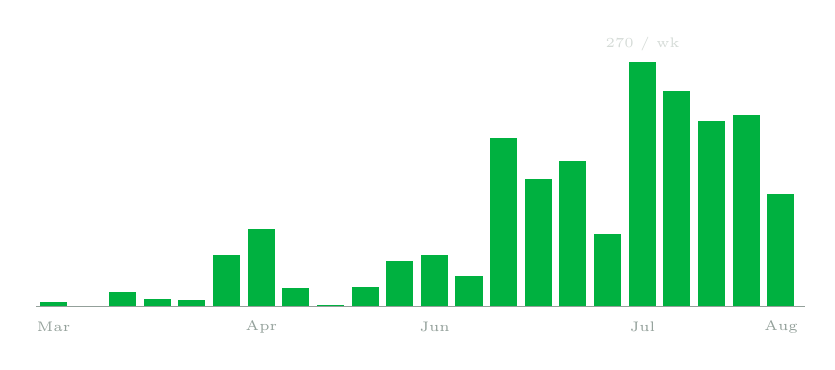
\begin{tikzpicture}[x=0.44cm,y=0.0115cm]
    \foreach [count=\i] \h in {5,1,17,9,8,57,86,21,2,22,51,57,34,186,141,161,81,270,238,205,212,125}
      \fill[ULGreen] (\i,0) rectangle (\i+0.78,\h);
    \draw[MutedGray] (0.9,0) -- (23.1,0);
    \node[font=\tiny,text=MutedGray] at (1.4,-22)  {Mar};
    \node[font=\tiny,text=MutedGray] at (7.4,-22)  {Apr};
    \node[font=\tiny,text=MutedGray] at (12.4,-22) {Jun};
    \node[font=\tiny,text=MutedGray] at (18.4,-22) {Jul};
    \node[font=\tiny,text=MutedGray] at (22.4,-22) {Aug};
    \node[font=\tiny,text=LightText,anchor=south] at (18.4,272) {270 / wk};
  \end{tikzpicture}

  \vspace{0.5ex}
  \begin{itemize}
    \item \textbf{1{,}989} commits in 22 weeks --- précis repo alone;
          autocatpath keeps its own history
    \item Eras read off the graph: MCP core $\to$ drafts + web UI $\to$
          quest factory, LLM router, taproot $\to$ deploy \& hardening
    \item Sustained by the dark factory: overnight workers + review gates,
          not heroics
  \end{itemize}
\end{frame}

% ---------- 17 · scoreboard ----------
\begin{frame}{Status scoreboard}
  \citefield{}
  \small
  \begin{columns}[T]
    \begin{column}{0.5\textwidth}
      \begin{itemize}\itemsep0.25ex
        \item[\sdone] Ingest + search + taproot
        \item[\sdone] Nanopublications: gated mint $\to$ sign $\to$ OTS
              $\to$ registry (first one public)
        \item[\sdone] Fisheye TOC / discovery layer
        \item[\sdone] autocatpath core (NEB, CHE, uncertainty)
        \item[\sdone] Pathway explorer + dossiers
        \item[\sdone] Quest / todo factory + review tiers
        \item[\sdone] Local LLM fleet (Macs + Sparks)
        \item[\sdone] Morning / evening briefs
        \item[\sdone] Citation export incl.\ EndNote traveling library
        \item[\sdone] Slab structure kind (ops, probes, diff)
      \end{itemize}
    \end{column}
    \begin{column}{0.5\textwidth}
      \begin{itemize}\itemsep0.25ex
        \item[\srough] One router, every model (first deploy + debug pending)
        \item[\srough] Argument graph \(\cdot\) categorizers \(\cdot\) Anki
        \item[\srough] Catalysis-DB import \(\cdot\) sim containers
        \item[\srough] Economics instrumentation
        \item[\srough] ICHEC national HPC: LLM burst (built, dark);
              sim / ML-potentials / DFT to follow
        \item[\sidea] Coverage audit \(\cdot\) evaluation suite
        \item[\sidea] Digests \(\cdot\) living paper
        \item[\sidea] Multi-member lab mode
      \end{itemize}
    \end{column}
  \end{columns}
\end{frame}

% ---------- 18 · next ----------
\begin{frame}{Next}
  \citefield{}
  \begin{itemize}
    \item Now: economics numbers (probe out), first evaluation metrics
          wired into the scoreboard
    \item Decisions pending: OC20 vs AQCat25 import; journal target
          (recommendation: \emph{Digital Discovery})
    \item Paper: living draft seeded from this deck; autocatpath JOSS
          companion
    \item Asks: [hardware / time / student --- fill in]
  \end{itemize}
\end{frame}

% ---------- 19 · references ----------
\begin{frame}{References}
  \citefield{}
  \scriptsize
  \begin{itemize}
    \item Farquhar, Kossen, Kuhn, Gal (2024). Detecting hallucinations in
          large language models using semantic entropy. \emph{Nature} 630,
          625--630. \doi{10.1038/s41586-024-07421-0}
    \item Shumailov, Shumaylov, Zhao, Papernot, Anderson, Gal (2024).
          AI models collapse when trained on recursively generated data.
          \emph{Nature} 631, 755--759. \doi{10.1038/s41586-024-07566-y}
    \item Gerstgrasser et al. (2024). Is model collapse inevitable?
          Breaking the curse of recursion by accumulating real and
          synthetic data. \emph{COLM 2024}.
          \href{https://arxiv.org/abs/2404.01413}{\texttt{arXiv:2404.01413}}
    \item Gottweis et al. (2026). Accelerating scientific discovery with
          Co-Scientist. \emph{Nature} 655, 487--496.
          \doi{10.1038/s41586-026-10644-y}
    \item autocatpath: \texttt{github.com/retospect/catpath} \(\cdot\)
          précis: \texttt{github.com/retospect/precis-mcp} ---
          both GPL-3.0-or-later
  \end{itemize}
\end{frame}

\end{document}
